\section{Progettazione logica}
\subsection{Stima del volume dei dati}
Si suppone che siano state giocate 10 partite alla quale hanno partecipato ogni volta 4 giocatori diversi. Le partite sono state giocate solo con l'espansione base (8 seguaci per giocatore e 62 tessere totali).
\medskip

\centerline{\begin{tabular}{ |l|c|c| }
\hline
\textbf{Concetto} & \textbf{Tipo} & \textbf{Volume} \\
\hline
Player & E & 40 \\
Participation & R & 40 \\
PlayerInGame & E & 40 \\
Having & R & 40 \\
Color & E & 10 \\
\hline
Meeple & E & 320 \\
Owning & R & 320 \\
Classification & R & 320 \\
BasicMeeple & E & 1 \\
ExpansionMeeple & E & 1 \\
Using & R & 1 \\
\hline
GameSet & E & 1.500 \\
Classification & R & 1.500 \\
BasicGameSet & E & 1 \\
ExpansionGameSet & E & 0 \\
Using & R & 0 \\
\hline
Game & E & 10 \\
Participation & R & 40 \\
Composition & R & 620 \\
Hosting & R & 10 \\
Using & R & 10 \\
\hline
Expansion & E & 4 \\
\hline
Server & E & 10 \\
Location & R & 10 \\
Region & E & 6 \\
Composition & R & 6 \\
Continent & E & 4 \\
Composition & R & 6 \\
CardinalPoint & E & 5 \\
\hline
\end{tabular}
\begin{tabular}{ |l|c|c| }
\hline
\textbf{Concetto} & \textbf{Tipo} & \textbf{Volume} \\
\hline
Tile & E & 620 \\
Classification & R & 620 \\
BasicTile & E & 18 \\
ExpansionTile & E & 7 \\
Using & R & 7 \\
Composition & R & 8.060 \\
\hline
TileSection & E & 8.060 \\
Composition & R & 8.060 \\
Classification & R & 8.060 \\
Placement & R & 200 \\
TileSectionType & E & 13 \\
Preceding & R & 12 \\
Composition & R & 325 \\
\hline
TileTypeConfiguration & E & 325 \\
Composition & R & 325 \\
Description & R & 325 \\
\hline
\end{tabular}}

\subsection{Descrizione delle operazioni principali e stima della frequenza}
Si suppone che ogni giorno vengano giocate 10 partite alla quale partecipano ogni volta 4 giocatori diversi. Le partite vengono sempre concluse nell'arco della giornata e si prevede che mediamente vengono giocate 70 tessere a partite.
\medskip

\centerline{\begin{tabular}{ |c|l|c| }
\hline
\textbf{Cod.} & \textbf{Operazione} & \textbf{Frequenza} \\
\hline
1 & Creare una nuova partita & 10 al giorno \\
\hline
2 & Visualizzare i server di gioco disponibili & 10 al giorno \\
\hline
3 & Visualizzare tutte le espansioni & 10 al giorno \\
\hline
4 & Creare un nuovo giocatore & 40 al giorno \\
\hline
5 & Visualizzare tutti i colori & 40 al giorno \\
\hline
6 & Visualizzare il giocatore corrente & 700 al giorno \\
\hline
7 & Visualizzare la tessera corrente & 700 al giorno \\
\hline
8 & Ruotare la tessera corrente & 300 al giorno \\
\hline
9 & Piazzare la tessera corrente & 700 al giorno \\
\hline
10 & Piazzare o rimuovere un seguace su una sezione di una tessera & 350 al giorno \\
\hline
11 & Visualizzare i seguaci disponibili ad un giocatore & 700 al giorno \\
\hline
12 & Assegnare dei punti ad un giocatore & 200 al giorno \\
\hline
13 & Aggiornare la tessera corrente & 700 al giorno \\
\hline
14 & Aggiornare il giocatore corrente & 700 al giorno \\
\hline
15 & Visualizzare le partire non concluse & 5 al giorno \\
\hline
16 & Visualizzare i giocatori di una partita & 70 al giorno \\
\hline
17 & Visualizzare le tessere piazzate in una partita & 5 al giorno \\
\hline
18 & Visualizzare le regioni in ordine di punteggio medio dei giocatori & 2 al mese \\
\hline
19 & Mostrare per ogni giocatore il numero di avversari con cui ha giocato & 4 all'anno \\
\hline
20 & Visualizzare per ogni regione l'espansione più giocata & 1 al mese \\
\hline
21 & Mostrare per ogni colore la probabilità statistica di vincere & 1 al giorno \\
\hline
\end{tabular}}

\subsection{Schemi di navigazione e tabelle degli accessi}

\subsection{Raffinamento dello schema}
\subsubsection*{Eliminazione delle gerarchie}
\medskip

\subsubsection*{Eliminazione degli attributi compositi}
(elimanzione dell'attributo composto Position e l'inserimento delle due coordinate)

\medskip
\subsubsection*{Eliminazione degli identificatori esterni}
Nello schema E/R sono state eliminate le seguenti relazioni:
\begin{itemize}
    \item Participation, importando name da players in players\_in\_game
    \item Participation, importando id da games in players\_in\_game
    \item Having, importando hex da colors in players\_in\_game
    \item Owning, importando player\_name e game\_id da players\_in\_game in meeples
    \item Composition, importando name da continents in regions
    \item Composition, importando name da cardinal\_points in regions
    \item Location, importando id da regions in servers
    \item Hosting, importando id da servers in games
    \item Using, reificata importando id da games e name da expansions
    \item Composition, importando id da games in tiles
    \item Placement, importando id da meeples in tile\_sections
    \item Composition, importando game\_id e order da tiles in tile\_sections
    \item Composition, importando id da gamesets in tile\_sections
    \item Preceding, importando name da tile\_section\_types in tile\_section\_types
    \item Composition, importando name da tile\_section\_types in tile\_types\_configurations
    \item Composition, importando name da gameset\_types in tile\_types\_configurations
    \item Description, importando name da tile\_types in tile\_types\_configurations
    \item Classification, importando name da meeple\_types in meeples
    \item Classification, importando name da tile\_section\_types in tile\_sections
    \item Classification, importando name da gameset\_types in gamesets
    \item Classification, importando name da tile\_types in tiles
    \item Using, importando name da expansions in tile\_types
    \item Using, importando name da expansions in gameset\_types
    \item Using, importando name da expansions in meeple\_types
\end{itemize}
In tile\_section\_types abbiamo scelto di importare due volte name da se stessa per avere sia la successiva che la precedente TileSection.

\medskip
\subsubsection*{Scelta delle chiavi primarie}
La maggior parte delle chiavi primarie sono già evidenziate in modo chiaro nello schema. Da notare l'entità Tile che è identificata tramite l'id della partita e l'ordine preciso in cui viene giocata. Per quanto riguarda l'entità TileSection questa è invece identificata tramite la Tile e il TileSectionType che è univoco all'interno di una Tile. Infine, l'entità TileTypeConfiguration è identificata con il TileType, il TileSectionType e un id aggiuntivo usato per distinguere i vari insiemi di GameSetType uguali presenti su una Tile di quel TileType. Questo è obbligatorio in quanto su una stessa Tile potrebbero esserci due GameSet con stesso GameSetType da considerare separati.

\subsection{Analisi delle ridondanze}

\subsection{Traduzione di entità e associazioni in relazioni}
\hspace{1.5em}players(\textbf{name})\newline

colors(\textbf{hex}, red, green, blue, name)\newline

games(\textbf{id}, server\_id, concluded)\newline
FK: server\_id REFERENCES servers(id)\newline

players\_in\_game(\textbf{player\_name}, \textbf{game\_id}, color\_hex, score, current, order)\newline
FK: player\_name REFERENCES players(name)\newline
FK: game\_id REFERENCES games(id)\newline
FK: color\_hex REFERENCES colors(hex)\newline

games\_expansions(\textbf{expansion\_name}, \textbf{game\_id})\newline
FK: game\_id REFERENCES games(id)\newline
FK: expansion\_name REFERENCES expansions(name)\newline

expansions(\textbf{name})\newline

meeple\_types(\textbf{name}, quantity, strength, expansion\_name)\newline
FK: expansion\_name REFERENCES expansions(name)\newline

meeples(\textbf{id}, owner\_player\_name, owner\_game\_id, type\_name, placed)\newline
FK: owner\_player\_name REFERENCES players\_in\_game(player\_name)\newline
FK: owner\_game\_id REFERENCES players\_in\_game(game\_id)\newline
FK: type\_name REFERENCES meeple\_types(name)\newline

gamesets(\textbf{id}, type\_name, points, closed)\newline
FK: type\_name REFERENCES gameset\_types(name)\newline

gameset\_types(\textbf{name}, starting\_points, endgame\_ratio, expansion\_name)\newline
FK: expansion\_name REFERENCES expansions(name)\newline

tile\_section\_types(\textbf{name}, next\_name*, previous\_name*)\newline
FK: next\_name REFERENCES tile\_section\_types(name)\newline
FK: previous\_name REFERENCES tile\_section\_types(name)\newline

tile\_sections(\textbf{type\_name}, \textbf{tile\_order}, \textbf{tile\_game\_id}, gameset\_id, meeple\_id*, closed)\newline
FK: type\_name REFERENCES tile\_section\_types(name)\newline
FK: tile\_order REFERENCES tiles(order)\newline
FK: tile\_game\_id REFERENCES tiles(game\_id)\newline
FK: meeple\_id REFERENCES meeples(id)\newline
FK: gameset\_id REFERENCES gamesets(id)\newline

tiles(\textbf{order}, \textbf{game\_id}, type\_name, rotation\_count, x\_coordinate*, y\_coordinate*, current)\newline
FK: type\_name REFERENCES tile\_types(name)\newline
FK: game\_id REFERENCES games(id)\newline

tile\_types(\textbf{name}, quantity, expansion\_name)\newline
FK: expansion\_name REFERENCES expansions(name)\newline

tile\_type\_configurations(id, \textbf{tile\_section\_type\_name}, \textbf{tile\_type\_name}, gameset\_type\_name, closed, pennant)\newline
FK: tile\_section\_type\_name REFERENCES tile\_section\_types(name)\newline
FK: tile\_type\_name REFERENCES tile\_types(name)\newline
FK: gameset\_type\_name REFERENCES gameset\_types(name)\newline

regions(\textbf{id}, continent\_name, cardinal\_point\_name*)\newline
FK: continent\_name REFERENCES continents(name)\newline
FK: cardinal\_point\_name REFERENCES cardinal\_points(name)\newline

continents(\textbf{name})\newline

cardinal\_points(\textbf{name})\newline

servers(\textbf{id}, region\_id, active, max\_games)\newline
FK: region\_id REFERENCES regions(id)

\subsection{Schema relazionale finale}
\begin{figure}[ht]
    \centering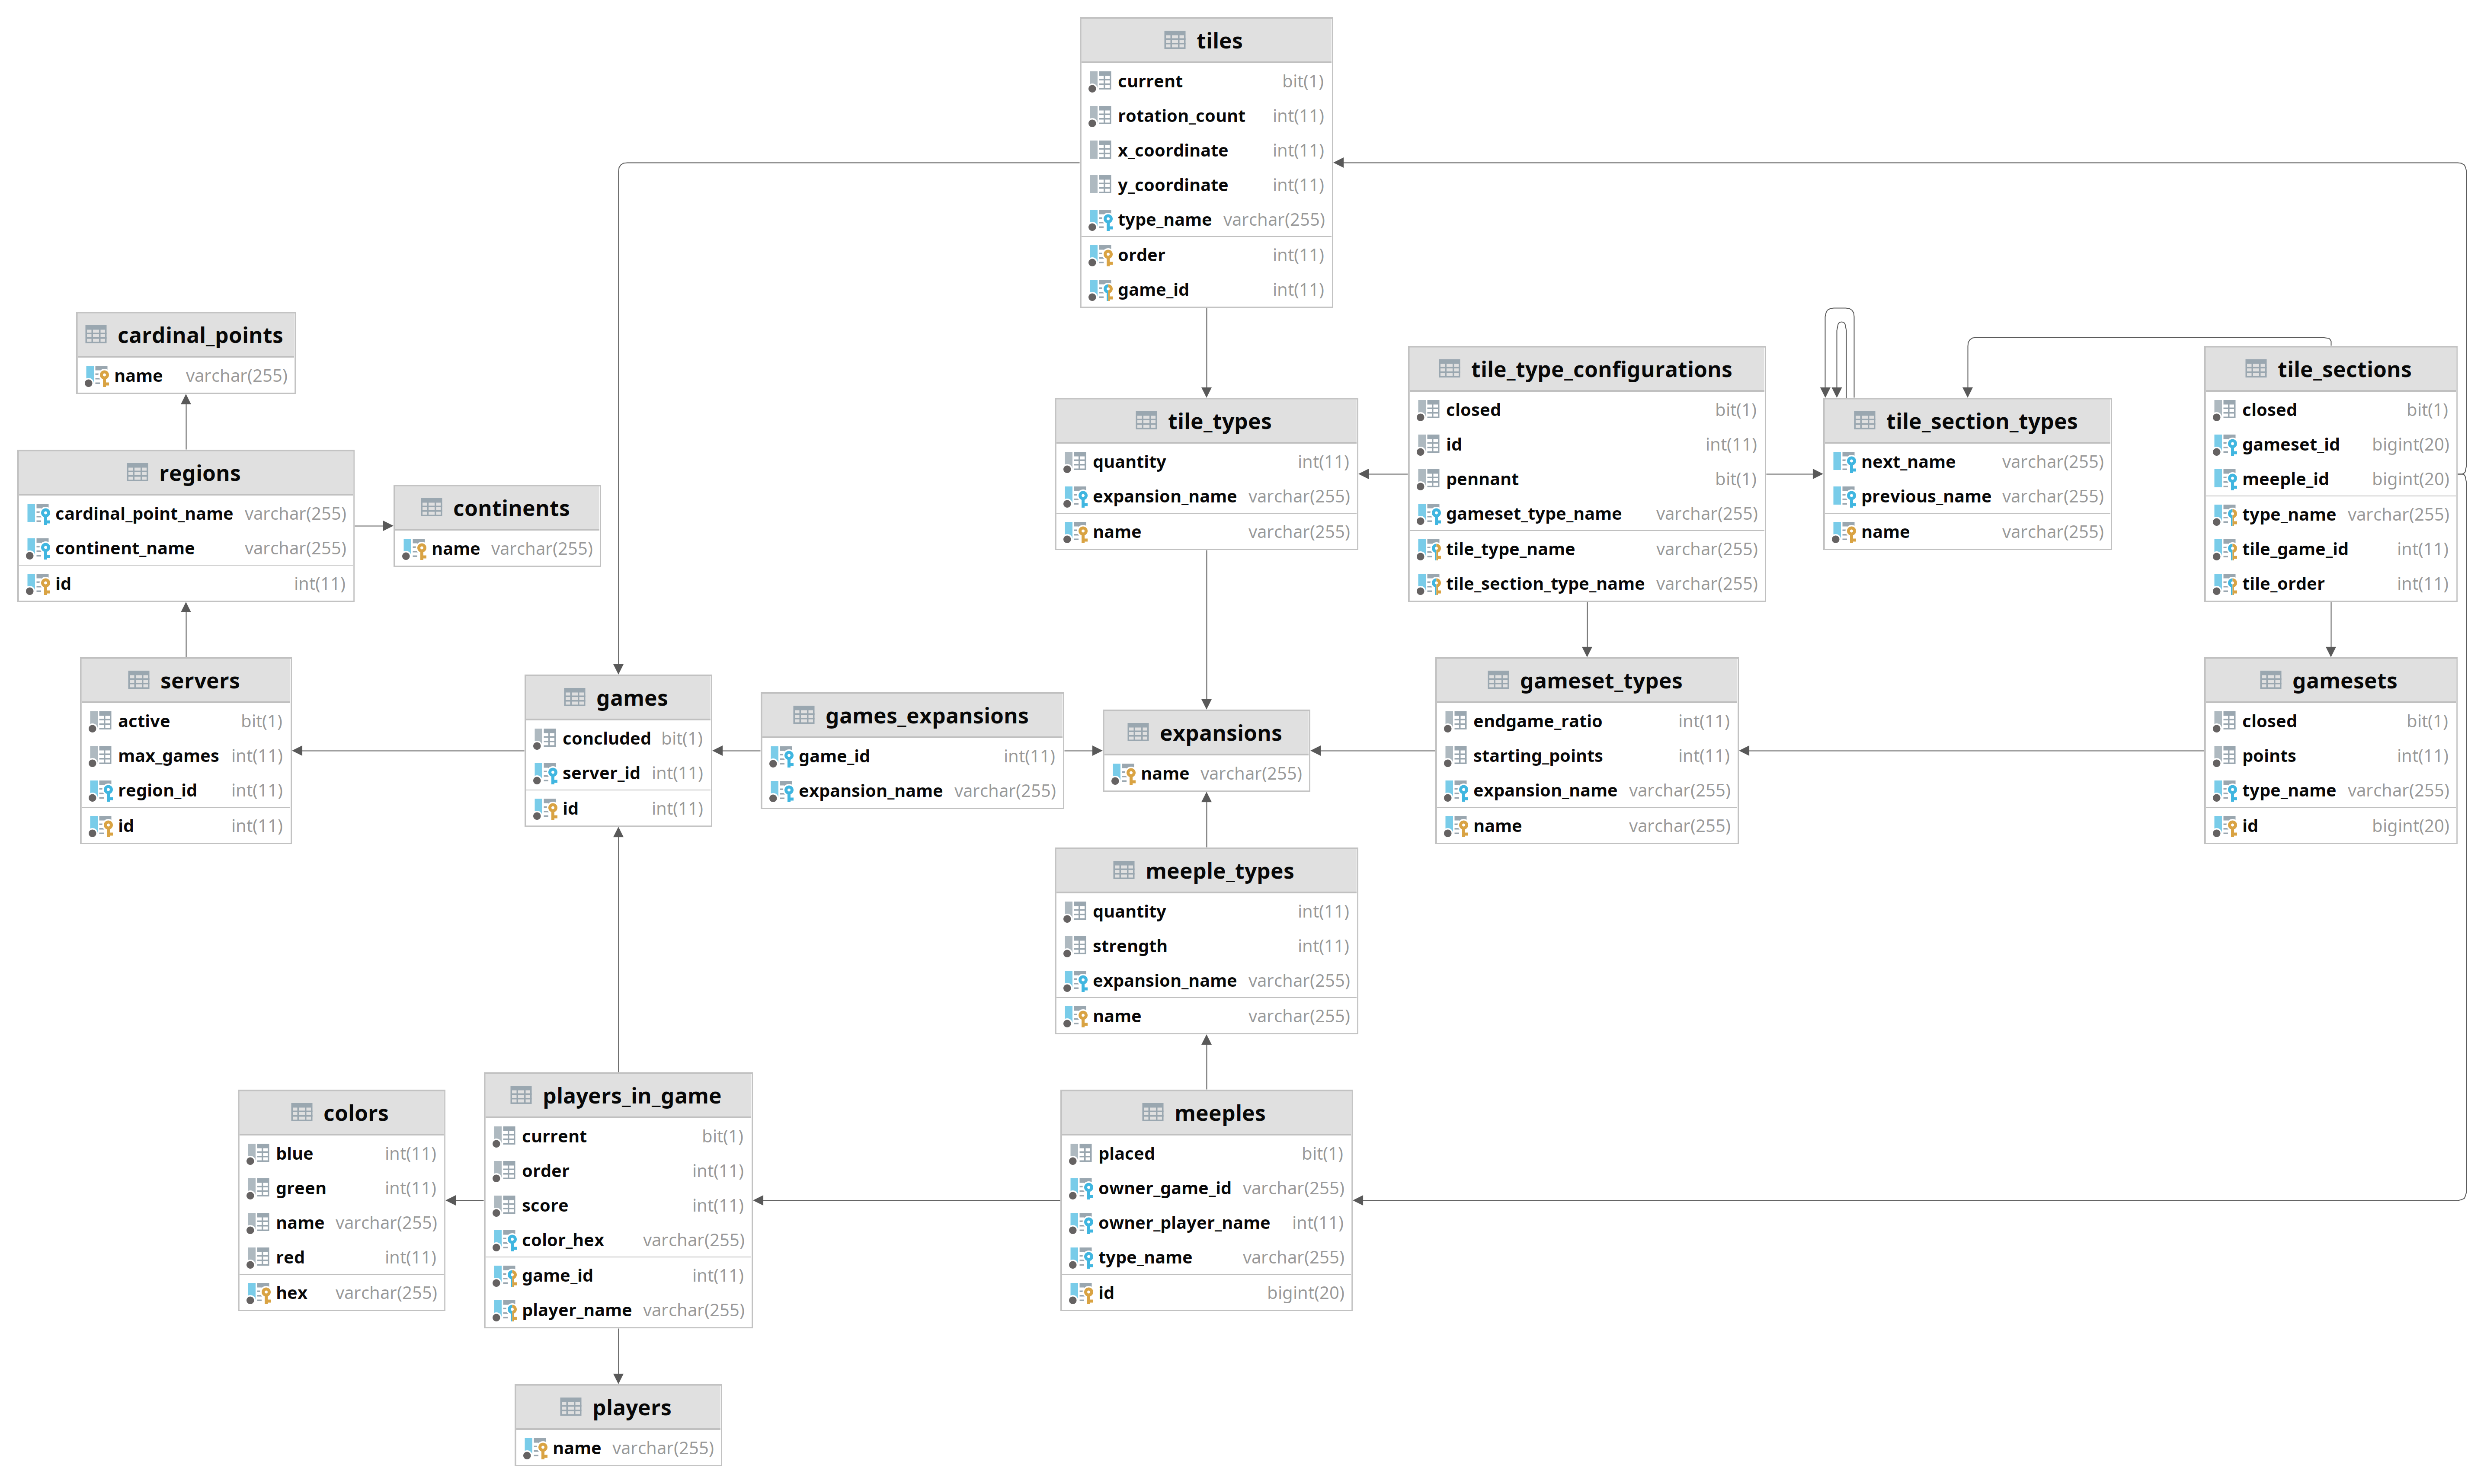
\includegraphics[scale=0.06]{images/Progettazione/relazionale.png}
    \caption{Schema concettuale finale.}
\end{figure}

\subsection{Traduzione delle operazioni in query SQL}
\subsubsection*{OP1 - Creare una nuova partita}
Nel caso in cui i giocatori scelti non esistano nel database vengono creati tramite l'operazione 4. Viene poi creata la partita assieme ai vari players\_in\_game che avranno come game\_id l'id della partita appena creata. Vengono poi creati i seguaci, le strutture e le tessere con le relative sezioni in accordo con le espansioni selezionate alla creazione del gioco.
\medskip

\begin{lstlisting}[style=sql]
    INSERT INTO games (concluded, server_id)
    VALUES (FALSE, ?);

    INSERT INTO players_in_game (current, `order`, score, game_id, player_name, color_hex)
    VALUES (FALSE, ?, 0, ?, ?, ?);

    INSERT INTO meeples (placed, owner_game_id, owner_player_name, type_name)
    VALUES (FALSE, ?, ?, ?);

    INSERT INTO gamesets (closed, points, type_name)
    VALUES (FALSE, 0, ?);

    INSERT INTO tiles (`order`, current, rotation_count, x_coordinate, y_coordinate, game_id, type_name)
    VALUES (?, FALSE, 0, null, null, ?, ?);

    INSERT INTO tile_sections (closed, type_name, tile_game_id, tile_order, gameset_id, meeple_id)
    VALUES (FALSE, ?, ?, ?, ?, null);
\end{lstlisting}

\subsubsection*{OP2 - Visualizzare i server di gioco disponibili}
Un server di gioco è disponibile solo se il numero di partite ancora in corso su quel server è inferiore al suo campo max\_games.
\medskip

\begin{lstlisting}[style=sql]
SELECT *
FROM servers AS s
WHERE active=true AND max_games > (SELECT COUNT(*)
    FROM games AS g
    WHERE g.server_ID=s.ID AND g.concluded = FALSE);
\end{lstlisting}

\subsubsection*{OP3 - Visualizzare tutte le espansioni}
\begin{lstlisting}[style=sql]
    SELECT *
    FROM expansions;
\end{lstlisting}

\subsubsection*{OP4 - Creare un nuovo giocatore}
\begin{lstlisting}[style=sql]
    INSERT INTO players (name)
    VALUES (?);
\end{lstlisting}

\subsubsection*{OP5 - Visualizzare tutti i colori}
\begin{lstlisting}[style=sql]
    SELECT *
    FROM colors;
\end{lstlisting}

\subsubsection*{OP6 - Visualizzare il giocatore corrente}
\begin{lstlisting}[style=sql]
    SELECT *
    FROM players_in_game
    WHERE game_id = ? AND current = TRUE;
\end{lstlisting}

\subsubsection*{OP7 - Visualizzare la tessera corrente}
\begin{lstlisting}[style=sql]
    SELECT *
    FROM tiles
    WHERE game_id = ? AND current = TRUE;
\end{lstlisting}

\subsubsection*{OP8 - Ruotare la tessera corrente}
Per ruotare la tessera corrente bisogna cambiare il tipo delle sezioni ad essa associate, essendo queste parte della chiave si è costretti a rimuoverle per poi re-inserirle aggiornate. Per ogni sezione della tessera corrente bisogna solo aggiornare l'attributo type\_name con il valore dell'attributo next\_name del tipo della sezione in questione, il resto rimane invariato.
\medskip

\begin{lstlisting}[style=sql]
    SELECT *
    FROM tile_sections
    WHERE tile_game_id = ? AND tile_order = ?;

    DELETE
    FROM tile_sections
    WHERE tile_game_id = ? AND tile_order = ?;

    -- Per ogni sezione di tile selezionata con la prima query
    INSERT INTO tile_sections (closed, type_name, tile_game_id, tile_order, gameset_id, meeple_id)
    VALUES (?, ?, ?, ?, ?, ?);
\end{lstlisting}


\subsubsection*{OP9 - Piazzare la tessera corrente}
\begin{lstlisting}[style=sql]
    UPDATE tiles
    SET x_coordinate = ?,
        y_coordinate = ?
    WHERE game_id = ? AND current = TRUE;
\end{lstlisting}

\subsubsection*{OP10 - Piazzare o rimuovere un seguace su una sezione di una tessera}
Nel caso della rimozione di un seguace è invece necessario impostare il relativo attributo placed a false. Inoltre, bisogna anche impostare a null l'attributo meeple\_id della sezione sulla quale era piazzato.
\medskip

\begin{lstlisting}[style=sql]
    UPDATE meeples
    SET placed = TRUE
    WHERE id = ?;

    UPDATE tile_sections
    SET meeple_id = ?
    WHERE type_name = ? AND tile_game_id = ? AND tile_order = ?;
\end{lstlisting}

\subsubsection*{OP11 - Visualizzare i seguaci disponibili ad un giocatore}
Un seguace è disponibile ad un giocatore se non è piazzato.
\medskip

\begin{lstlisting}[style=sql]
    SELECT *
    FROM meeples
    WHERE owner_player_name = ? AND owner_game_id = ? AND placed = FALSE;
\end{lstlisting}

\subsubsection*{OP12 - Assegnare dei punti ad un giocatore}
\begin{lstlisting}[style=sql]
    UPDATE players_in_game
    SET score = ?
    WHERE game_id = ? AND player_name = ?;
\end{lstlisting}

\subsubsection*{OP13 - Aggiornare la tessera corrente}
Il valore della wildcard per l'attributo order della seconda query si ricava incrementando di 1 l'attributo order della tessera che era prima corrente.
\medskip

\begin{lstlisting}[style=sql]
    UPDATE tiles
    SET current = FALSE
    WHERE game_id = ? AND current = TRUE;

    UPDATE tiles
    SET current = TRUE
    WHERE game_id = ? AND order = ?;
\end{lstlisting}

\subsubsection*{OP14 - Aggiornare il giocatore corrente}
Il valore della wildcard per l'attributo order della seconda query si ricava incrementando di 1 l'attributo order del giocatore che era prima corrente e applicandogli il modulo con il numero di giocatori della partita.
\medskip

\begin{lstlisting}[style=sql]
    UPDATE players_in_game
    SET current = FALSE
    WHERE game_id = ? AND current = TRUE;

    UPDATE players_in_game
    SET current = TRUE
    WHERE game_id = ? AND order = ?;
\end{lstlisting}

\subsubsection*{OP15 - Visualizzare le partire non concluse}
\begin{lstlisting}[style=sql]
    SELECT *
    FROM games
    WHERE concluded = FALSE;
\end{lstlisting}

\subsubsection*{OP16 - Visualizzare i giocatori di una partita}
\begin{lstlisting}[style=sql]
    SELECT *
    FROM players_in_game
    WHERE game_id = ?;
\end{lstlisting}

\subsubsection*{OP17 - Visualizzare le tessere piazzate in una partita}
\begin{lstlisting}[style=sql]
    SELECT *
    FROM tiles
    WHERE game_id = ? AND x_coordinate IS NOT NULL AND y_coordinate IS NOT NULL;
\end{lstlisting}

\subsubsection*{OP18 - Visualizzare le regioni in ordine di punteggio medio dei giocatori}
In questo caso vengono considerate solo le partite concluse.
\medskip

\begin{lstlisting}[style=sql]
SELECT R.id, AVG(P.score) AS AveragePlayerScore
FROM ((regions R INNER JOIN servers S on R.id = S.region_id) INNER JOIN games G ON S.id = G.server_id) INNER JOIN players_in_game P ON G.id = P.game_id
WHERE G.concluded = TRUE
GROUP BY R.id
ORDER BY AveragePlayerScore DESC;
\end{lstlisting}

\subsubsection*{OP19 - Mostrare per ogni giocatore il numero di avversari con cui ha giocato}
Nella subquery per ogni giocatore si conta con quanti altri giocatori diversi e distinti ha giocato.
\medskip

\begin{lstlisting}[style=sql]
SELECT P.player_name, (SELECT COUNT(DISTINCT P2.player_name) AS EnemiesCount
    FROM players_in_game P2 INNER JOIN games G2 on P2.game_id = G2.id
    WHERE G2.id IN (SELECT DISTINCT P3.game_id
        FROM players_in_game P3
        WHERE P3.player_name = P.player_name) AND P2.player_name <> P.player_name) AS EnemiesCount
FROM players_in_game P INNER JOIN games G on P.game_id = G.id
GROUP BY P.player_name
ORDER BY EnemiesCount DESC;
\end{lstlisting}

\subsubsection*{OP20 - Visualizzare per ogni regione l'espansione più giocata}
Per questa operazione si è deciso di non considerare l'espansione base in quanto viene usata in ogni partita. Nella subquery per ogni regione si conta in quante partite è stata usata ogni espansione. Nella query esterna si seleziona solo l'espansione più giocata per ogni regione.
\medskip

\begin{lstlisting}[style=sql]
SELECT SQ.id, SQ.expansion_name, MAX(SQ.GamesCount) AS MaxGamesCount
FROM (SELECT R.id, GE.expansion_name, COUNT(GE.expansion_name) AS GamesCount
    FROM ((regions R INNER JOIN servers S on R.id = S.region_id) INNER JOIN games G ON G.server_id = S.id) INNER JOIN games_expansions GE ON GE.game_id = G.id
    WHERE GE.expansion_name <> 'Basic'
    GROUP BY R.id, GE.expansion_name) AS SQ
GROUP BY SQ.id
ORDER BY SQ.id ASC;
\end{lstlisting}

\subsubsection*{OP21 - Mostrare per ogni colore la probabilità statistica di vincere}
TODO: Davide. Non so che hai usato lì nella select lol
\medskip

\begin{lstlisting}[style=sql]
SELECT c.name, (SUM(CASE WHEN pig.Score = max_scores.max_score THEN 1 ELSE 0 END) / COUNT(*)) AS WinProbability
FROM colors c JOIN players_in_game pig ON c.hex = pig.color_hex JOIN (SELECT game_id, MAX(Score) AS max_score
FROM players_in_game
GROUP BY game_id) max_scores ON pig.game_id = max_scores.game_id JOIN games g ON pig.game_id = g.id
WHERE g.concluded = TRUE
GROUP BY c.hex, c.name;
\end{lstlisting}
